\subsection{Схема Блома}\label{section-bloms-scheme}\index{схема!Блома|(}
\selectlanguage{russian}

Схема Блома (\langen{Rolf Blom},~\cite{Blom:1984, Blom:1985}) используется в протоколе HDCP\index{протокол!HDCP} (\langen{High-bandwidth Digital Content Protection}) для предотвращения копирования высококачественного видеосигнала. Предполагается, что некоторый доверенный центр распределит ключи таким образом, что легальные производители видеокарт, мониторов высокого разрешения и других компонент будут передавать видеоконтент по защищённому каналу, а <<пиратские>> устройства не смогут эти данные перехватить, и, например, записать на другой носитель.

На этапе инициализации доверенный центр выбирает симметричную матрицу $D_{m,m}$ над конечным полем $\GF p$. Для присоединения к сети распространения ключей, новый участник либо самостоятельно, либо с помощью доверенного центра выбирает новый открытый ключ (идентификатор) $I_i$, представляющий собой вектор длины $m$ над $\GF p$. Доверенный центр вычисляет для нового участника закрытый ключ $K_i$:
\begin{equation}
	K_i = D_{m,m} I_i.
	\label{eq:blom_center_matrix}
\end{equation}

Симметричность матрицы $D_{m,m}$ доверенного центра позволяет любым двум участникам сети создать общий сеансовый ключ. Пусть Алиса и Боб -- легальные пользователи сети, то есть они обладают открытыми ключами $I_A$ и $I_B$ соответственно, а их закрытые ключи $K_A$ и $K_B$ были вычислены одним и тем же доверенным центром по формуле~\ref{eq:blom_center_matrix}. Тогда протокол выработки общего секретного ключа выглядит следующим образом (рис.~\ref{fig:key_distribution-bloms-scheme}).

\begin{figure}
    \centering
    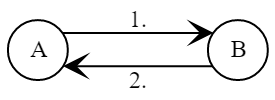
\includegraphics[width=0.5\textwidth]{pic/key_distribution-bloms-scheme}
    \caption{Взаимодействие участников в схеме Блома\label{fig:key_distribution-bloms-scheme}}
\end{figure}

\begin{protocol}
    \item[(1)] $Alice \to \left\{ I_A \right\} \to Bob$
    \item[(2)] Боб вычисляет $K_{BA} = K^T_B I_A = I^T_B D_{m,m} I_A$.
    \item[{}] $Bob \to \left\{ I_B \right\} \to Alice$
    \item[(3)] Алиса вычисляет $K_{AB} = K^T_A I_B = I^T_A D_{m,m} I_B$.
\end{protocol}

Из симметричности матрицы $D_{m,m}$ следует, что значения $K_{AB}$ и $K_{BA}$ совпадут, они же и будут являться общим секретным ключом для Алисы и Боба. Этот секретный ключ будет свой для каждой пары легальных пользователей сети.

Присоединение новых участников к схеме строго контролируется доверенным центром, что позволяет защитить сеть от нелегальных пользователей. Надёжность данной схемы основывается на невозможности восстановить исходную матрицу. Однако для восстановления матрицы доверенного центра размера $m \times m$ необходимо и достаточно всего $m$ пар линейно независимых открытых и закрытых ключей. В 2010-м году компания Intel, которая является <<доверенным центром>> для пользователей системы защиты HDCP, подтвердила, что криптоаналитикам удалось найти секретную матрицу (точнее, аналогичную ей), используемую для генерации ключей в упомянутой системе предотвращения копирования высококачественного видеосигнала.

\index{схема!Блома|)}